% !Mode:: "TeX:UTF-8"

\documentclass[UTF8,a4paper]{article}
\usepackage{ctex}
\usepackage[sort&compress,numbers]{natbib}
\usepackage{ccaption} 
\usepackage{booktabs}
\usepackage{geometry}
\usepackage{titlesec}
\usepackage{url}
\usepackage[font={small,bf}]{caption}
\usepackage[yyyymmdd]{datetime}
\geometry{left=3.18cm,right=3.18cm,top=2.54cm,bottom=2.54cm}
\pagenumbering{gobble}
\renewcommand\refname{Reference}
\usepackage{graphicx}
\usepackage{subfigure}
\usepackage[ruled,lined,commentsnumbered,linesnumbered]{algorithm2e}
\usepackage{amsmath}
\usepackage[pdftex]{hyperref} 




\titleformat*{\section}{\songti\zihao{4}\bfseries}
\titleformat*{\subsection}{\heiti\zihao{5}\bfseries}
\titleformat*{\subsubsection}{\kaishu\zihao{5}\bfseries}

\newenvironment{csmtAbstract}{\noindent \kaishu \small {\bfseries Abstract:}}{}
\newenvironment{keywords}{\small \noindent{\bfseries Key Words:}}{}
\newcommand{\weizhuProject}[2] {\noindent{\bfseries Recieved Date:~{\small \today}} \newline {\bfseries \indent ~~Support Project:} {\small #1} \newline {\bfseries \indent ~~Author:} {\small #2}}
\newcommand{\weizhu}[1] {\noindent{\bfseries Recieved Date:\today} \newline {\bfseries \indent ~~Author:} #1}
\renewcommand{\figurename}{Fig.}
\renewcommand{\tablename}{Tab.}
\renewcommand{\dateseparator}{--}

\newcommand*{\affaddr}[1]{{ \small {#1}}} 
\newcommand*{\affmark}[1][*]{\textsuperscript{#1}}

\makeatletter
\renewcommand\@maketitle{%
	\hfill
	\begin{minipage}{0.95\textwidth}
		\vskip 2em
		%\let\footnote\thanks 
		% Please select the applicable commands for foot notes
		%{\centering \bfseries \zihao{3} \@title \thanks{\weizhuProject{Project Title}{Corresponding Author (1900--), M/F, Academic Degree, Academic Title, E-mail}}} \par } %For those funded by a grant
		{\centering \bfseries \zihao{3} \@title \par}%\thanks{\weizhu{Corresponding Author (1900--), M/F, Academic Degree, Academic Title, E-mail}} \par } %For those are not funded by a specific grant
		\vskip 2em
		{\centering \zihao{5} \textbf{\@author} \par}
	\end{minipage}
	\vskip 2em \par
}
\makeatother

%\title{A template for China Sound and Music Technology (CSMT) conference}
\title{Humanoid Robot Dance Control \\ over Real-Time Music Stimulation \\ [1ex] \begin{large} AU332 Project Final Report \end{large} }

\author{%
	{Jingwei Zhao,  Zhengbao He}\\
	\affaddr{Shanghai Jiao Tong University, Shanghai, China}\\
	\affaddr{\{zhaojw, lstefanie\}@sjtu.edu.cn}\\
	%\affaddr{\affmark[2]Affliation 2,City~~Post Code}\\
}

\begin{document}
	
	\maketitle
	
	\begin{csmtAbstract}
		In this project, we implement a novel dance control system for humanoid robot over real-time music stimulation. We generate dance motions for the robot from RGB human dance videos by estimating the 3D human pose, which are further analytically mapped to corresponding joint angles to actuate the robot. With a motion base established in this way, we choreograph for the robot by selecting motions following a Markov Chain rule. To synchronize the motions to the music beats, we apply beat tracking algorithms in real time to extract beat claims as reference, and adjust the dance speed by feeding the motion-beat error into a PID controller. We test and evaluate our control system with the virtual robot Nao in the CoppeliaSim platform, which not only demostrates varied and visually pleasing dance motion sequences while keeping itself stable and balanced, but also displays a tight synchronization between the motions and music beats.
	\end{csmtAbstract}
	
	\begin{keywords}
		Humanoid Robot, Dance Control, Real-Time Music Stimulation
	\end{keywords}
	
	\section{Introduction}
	
	\noindent With the emergence of humanoid robots, there has been more and more instances where robots imitate human activities and interact with humans. Related work includes facial expression imitation\cite{ge2008facial}, human pose imitation\cite{zhang2018real, lei2015whole, zhangreal}, and human motion imitation\cite{kim2009stable, nakaoka2003generating, koenemann2014real}, etc. Since dance, as a classical performance art form, has been part of human social interaction for multiple millennia, enabling robots to imitate human dance has also become an actual field of research.

	There have been various contributions to the field of dancing robots. Early work such as \cite{geppert2004qrio, nakaoka2005task} actuate their robots to display impressive dancing capabilities by precisely pre-programming the sequence and timing of dancing motions (i.e., choreography) to a set of fixed musical pieces. However, they cannot respond to external musical stimulation as humans do. As for \cite{crick2006synchronization, bock2016robod, murata2008robot, schollig2010synchronizing}, their robots dance to external auditory or visual sitimulations, but are limited with single, periodic dance motions. 
	
	Besides motion design, the hardware and software delay presents another difficulty in controlling robot dance. Specifically, the robot's motion output tends to lag the input due to delays in arithmetic operations and data transmission. To stress this problem, \cite{bi2018real} combines a feedback PID controller with a feedforward lookup-table-based controller to synchronize the key frames of dancing motions to the music beats. This work also implements non-programmed choreography in correspondence with real-time music stimulation, but each of its motion primitives is still pre-programed, and the robot used here, namely, ANYMal\cite{hutter2016anymal}, is not humanoid.

	Our goal with this project is to enable a humanoid robot dance to real-time music stimulation, with non-programmed dancing motions which can be easily generated, and which are both varied and visually pleasing. The robot we select here is Nao produced by Softbank Robotics. Algorhithms are tested in the CoppeliaSim\cite{rohmercoppeliasim} platform, which is the newest version of Vrep\cite{rohmer2013v}. 
	
	To let the robot dance in a non-programmed way, we utilize 3D human pose estimation to extract 3D human pose of dancers from videos. The 3D pose is later mapped to corresponding robot joint angeles in an analytical way so that the robot can imitate the dancing motions. Since information about ankle joints are not recorded in the 3D human pose, we further analytically keep the robot's feet always parallel to the ground. This also keeps the robot in static stability, thus we can let it imitate more sophisticated motions.

	We set a motion base for the robot by extracting dancing poses from a number of videos. Each motion is consisted of a number of motion frames, which corresponds to the video frames from which the motions are extracted. To let the robot dance with real-time music, we follow \cite{bi2018real} and take advantage of the beat tracking algorhthms implemented by \cite{bock2014multi} to extract real-time music beats. To choreograph, we select dancing motions in an improvised way from the motion base with a Markov Chain rule. To synchronize the motions with the beats, we implement a PID controller in a feedback path to let the robot follow the music tightly. 

	In order to further stress the influence of time delay due to data transmission, we pack our whole control system into three mutually communicating processes, each taking charge of specific tasks. These processes are, namely, Beat Extractor, Motion Selector, and Speed Controller and Motion Actuator, respectively. An overall diagram is shown in Figure \ref{overall}.

	\begin{figure}[htb]
		\centering
		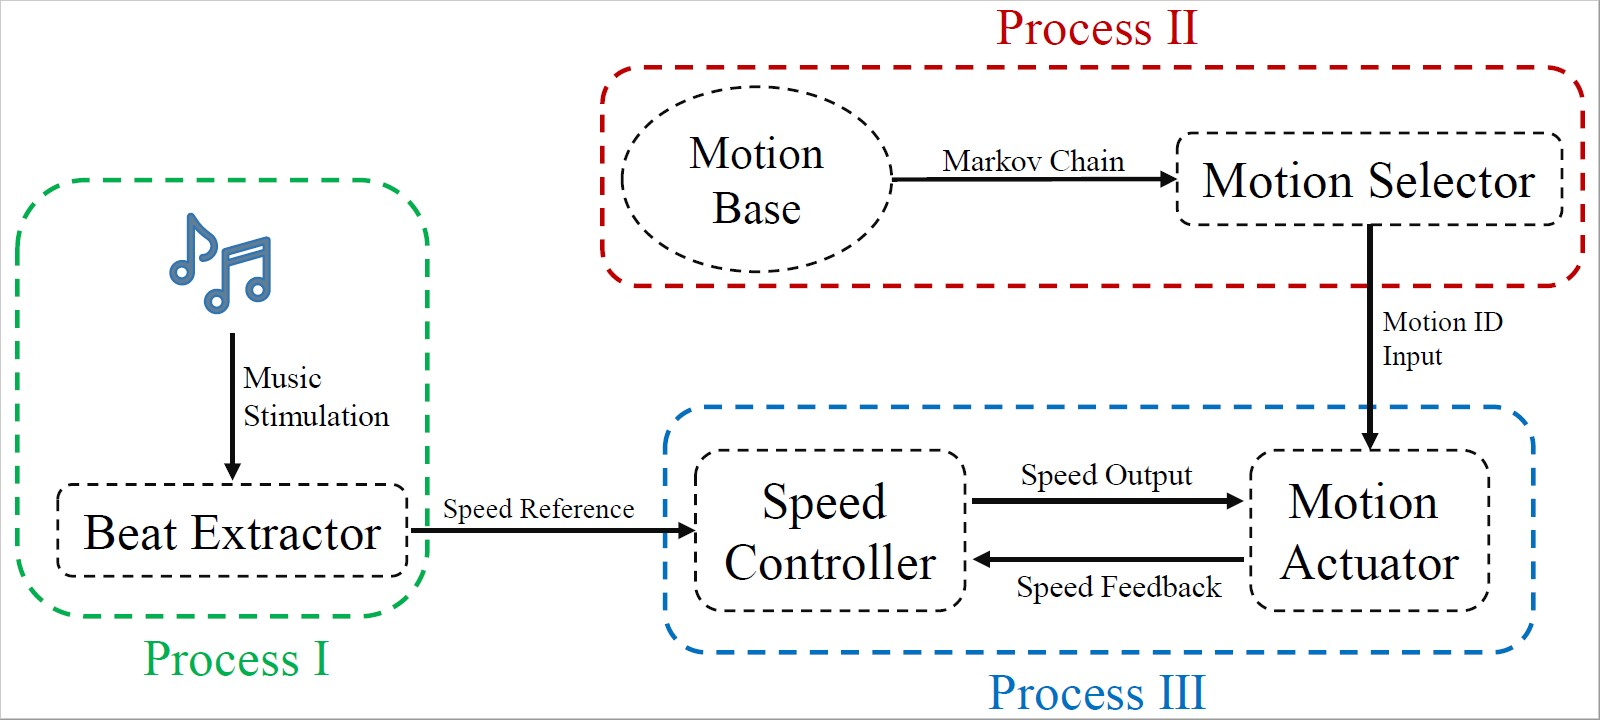
\includegraphics[scale=0.6]{overall_diagram.pdf}
		\caption{Overall Diagram of the Robot Dance Control System}
		\label{overall}
	\end{figure}

	The rest of this report is structured as follow. We introduce our work in Section \ref{section2}. Specifically, motion generation, motion selection, and speed control are introcuced in Section \ref{motion_generate}, \ref{motion_selection}, and \ref{speed} respectively. In Section \ref{section3}, we integrate each part, and evaluate the overall performance of our dance control system with robot Nao in the CoppeliaSim platform. Finally, we discuss our contribution and weakness in Section \ref{section4}.
	
	\section{Our Work}\label{section2}

	\subsection{Motion Generation}\label{motion_generate}

	\noindent In this part, we introduce the way we generate dance motions for the robot. We first estimate 3D human pose from dancing videos, and then map the pose locations into robot joint angles. A motion base is established by applying this process to many dance video clips. Each motion consists of a number of motion frames which are corresponding to the video frames from which they are extracted. The merit of our method is that, once the pipline is built, few codes are  needed for the generation of new motions. Details are illustrated as follow.

	\subsubsection{3D Human Pose Estimation}

	\noindent We estimate 3D human pose from RGB videos, most of which are solo dance episodes collected from YouTube. Specifically, for each video frame, we first crop the dancer out with Yolo v3\cite{redmon2018yolov3} by detecting the 'person' label, and then feed the detected image patch to ResPoseNet raised by \cite{moon2019camera} for 3D human pose estimation.
	
	The reason why we use Yolo to detect the dancer before pose estimation is that it helps ResPoseNet to concentrate on the dancer by putting the dancer in a whole image patch. Thus the 3D pose we obtain can be more accurate. With this method, we can also select certain dancer from multi-person dance videos to estimate poses, because Yolo v3 supports multi-target detection. However, We haven't tried such multi-person videos because we have found a number of good-quality solo dance ones. Thus we just input these videos, obtain the most confident framewise detection patch from Yolo, and then feed the detection to ResPoseNet for 3D human pose estimation. This further helps keeping a higher estimation accuracy. The whole procedure for this part is illustrated in Figure \ref{motion}.

	\begin{figure}[htb]
		\centering
		\includegraphics[scale=.7]{pose_estimation.pdf}
		\caption{Procedure of 3D Human Pose Estimation}
		\label{motion}
	\end{figure}

	\subsubsection{Mapping from Pose to Angle}

	\noindent Obtaining the pose information for each dance motion frame only partly solves our problem, because the 3D pose cannot be directly used to actuate the robot. In our project, to actuate Nao, we have to map the pose to Nao's joint angles. Nao has totally 25 free joints throughout its body. Since what we focus on is mapping dance motions, we neglect the joints for the neck, wrist, and fingers for simplicity. However, the rest work is still a rather huge systematic procudure.

	For mapping to the angles of Nao's joints of shoulders, elbows, hips, and knees, we follow \cite{lei2015whole} and implement an anylitical mapping method. Specifically, for each motion frame, each pose key point on the limbs can find its corresponding joint on Nao. By expressing the links as vectors from one key point to another, and applying dot and cross multipication with each other, the angles between two adjacent links can be obtained, and this angle can easily find its mapping to Nao's body joint angles. In practice, we found that the mapped results for the shoulder pitch angles tend to be very large. After confirming that the mapping method was correctly implemented, we concluded that this phenomenon should have something to do with ResPoseNet's own features. As a result, we multiply a factor smaller than one to these angles in order to keep visually pleasing dance motions.

	Another problem to tackle is that, the information for ankel joint angles are not recorded in the 3D human pose. Fortunately, we have the prior heuristic that the robot should keep stable and ballanced when making each dance motion. As a result, we try to keep its feet always parallel to the ground. To do so, we first simplify and model Nao's lower limbs analytically.Because it is rather difficult to do the modeling in 3D space, we map the 3D space into a vertical and a horizontal 2D plane for simplification. This mapping is kind of approximation, and the value we obtain could deviate from the true value, but the results we get in practice is quite feasible. 

	For example, in the instance of Figure \ref{limbs}, we model Nao's lower limbs (inside the black box), and get the approximation in Figure \ref{mapping}. $l_1$ and $l_2$ are the distances from Nao's hip joints to ankle joints projectd to the vertical plane, and $RHR$ and $LHR$ are the angles of {\itshape RightHipRoll} and {\itshape LeftHipRoll}, respectively.
	
	\begin{figure}[!h] \centering    
		\subfigure[Analytical Model] {
			\label{mapping}     
		\includegraphics[width=0.3\columnwidth]{ankle_mapping_2.pdf}
		}     
		\subfigure[Nao's Lower Limbs] { 
		\label{limbs}     
		\hspace{.5in}
		\includegraphics[width=0.34\columnwidth]{ankle_mapping_1.pdf}     
		}    
		\caption{Analytical Model for Ankle Joint Mapping}     
		\label{ankle}     
	\end{figure} 

	To control Nao's ankle joints while keeping it stable and ballenced, we need to obtain the value of $\theta_1$ and $\theta_2$ in Figure \ref{mapping}. And analytically,  we have:

	\begin{equation}
		\theta_1 = \arctan\left(\frac{\sin(LHR - RHR)}{\frac{a+l_1}{b+l_2}-\cos(LHR-RHR)} \right)
	\end{equation}

	\begin{equation}
		\theta_2 = \arctan\left(\frac{\sin(LHR - RHR)}{\frac{b + l_2}{a + l_1}-\cos(LHR-RHR)} \right)
	\end{equation}

	With $\theta_1$ and $\theta_2$, we can calculate corresponding values for the joint angle {\itshape RightAnkleRoll} and {\itshape LeftAnkleRoll}. A similar method can be applied to getting another pair of angles, namely, {\itshape RightAnklePitch} and {\itshape LeftAnklePitch}. In this way, we keep Nao's feet always parallel to the ground. Thus Nao can maintain stability while making each dance motion.

	In practice, probabily due to the deviation brought by our approximation, the robot could still fall down when the motion is fierce. So we limit the range of angle {\itshape RightKneePitch} and {\itshape LeftKneePitch}, and let Nao dance mainly along the vertical 2D plane. In this way, we can let Nao make both visually pleasing and stable and ballanced dance motions.

	\subsection{Motion Selection}\label{motion_selection}

	\noindent With the process introduced in the last part, a motion base is established by applying the algorithms to many dance video clips. Each motion consists of a number of motion frames which are corresponding to the video frames from which they are extracted.
	
	While we try to make our robot dance with varied motions, the motion sequence or choreography it follows should be logical in some sense. For example, certain motions may have a symmetric counterpart, and a left motion should be followed by a corresponding right motion in this case. Also, it may be resaonable to repeat certain motions several times, while not reasonable for other motions. As a result, specific features should be concidered for each motion when deciding which motion to choose next from the motion base.

	In our practice, for each motion with ID $n$, we set the following features:

	\begin{itemize}
		\item $BPS_n$: $BPS$ is abbreviation for $BeatPerSecond$. This feature is an interval which designates the bound of music tempo at which motion $n$ can run. Currently, the music clips we use to test our algorithms are of similar tempi, which are between this interval for all the motions. So we have not brought this feature into use yet. In our future work, we will rely on this feature to filter potential motions which could detereorate the robot's stability at certain tempo intervals.

		\item $Repeat_n$: This feature is the probability for which the next motion will repeat the current one. It ranges from 0 to 1, where 0 indicates that motion $n$ will never repeat itself, and 1 indicates that motion $n$ will always repeat itself once trigered. Currently, most of our motions have this value ranging from 0 to 0.5.

		\item $Symmetric_n$: This feature could be an integer number or the bollean value $False$. $False$ indicates that motion $n$ does not have a symmetric counterpart. An integer number indicates motion $n$ is symmetrc, and the number is extactly the ID of the corresponding symmetric motion. In practice, we follow the rule that left is prior to right, and we always assign odd ID to left motions and even ID to right motions in order to tell different cases. We let a left motion ($n$ is odd) jump to its right counterpart $Symmetric_n$ with probability = 1 ($Repeat_n=0$), and let a right motion ($n$ is even) jump back to its left counterpart $Symmetric_n$ with probability = $Repeat_n$.

		\item $FPB_n$: $FPB$ is abbreviation for $FramePerBeat$. This is an positive number which indicates the average number of frames between two consecutive key motion frames, where the 'key motion frames' are defined as the motion frames aligned with the beat of the soundtrack of its originated video. This feature is used to control the motion actuating speed, and will be illustrated in the next part.
	\end{itemize}

	Considering the features shown above, we establish our motion selector as a probabilistic model. Such a model does not pre-program the choreography with candidate motions, but generate motion sequence in an immprovised way. In this way, our robot can dance in varied patterns. Specifically, the motion selection process is designed as a Markov Chain. A Markov Chain is a sequence of discrete random variables
	$X_1$, $X_2$, $X_3$, $\ldots$ with transition probabilities of the next state given by the current one, i.e.,

	\begin{equation}
		P(X_{n+1}=x|X_1=x_1, X_2=x_2, \ldots, X_n=x_n) = P(X_{n+1}=x|X_n=x_n)
	\end{equation}

	The possible values $x_1$, $x_2$, $\ldots$, $x_i$ of $X_n$ are candidates of motion IDs for the $n^{th}$ motion. The transition probability $P(X_{n+1}=x_i|X_n=x_j)$ for the $n^{th}$ motion is determined by the features $BPS_{n}$, $Repeat_{n}$, $Symmetric_{n}$, and the current tempo of the music $BPS_{music}$. Conceptually, We impliment our motion selector as shown in Algorithm \ref{selector}, where the motionBuffer $Q$ is a data trasmission queue from Motion Selector to Motion Actuator. While the former puts selected motion ID in, the latter takes it out when a new motion is wanted.

		\begin{algorithm}[!h]
			\caption{Algorithm of Motion Selector}
			\label{selector}
			\KwIn{ motionBase $\textbf{B}$, initialMotion ID $\textbf{n}=0$, motionBuffer $\textbf{Q}$}
			\KwResult{Iterate and update $\textbf{n}$}
			$\textbf{Q}\leftarrow\textbf{n}$\;
			\While{Dance not terminated}
			{
				\If{$\textbf{Q}$ is empty}
				{
					$BPS_n, Symmetric_n, Repeat_n \leftarrow features(\text{motion }\textbf{n}$)\;
					\If{$Symmetric_n \neq False$ and $Symmetric_n$ is divisible by 2}
					{
						$\textbf{n} \leftarrow Symmetric_n$\;
					}
					\If{$Symmetric_n \neq False$ and $Repeat_n \neq 0$}
					{
						$\textbf{n} \leftarrow Symmetric_n$ with probability $Repeat_n$\;
					}
					\If{$Symmetric_n = False$ and $Repeat_n \neq 0$}
					{
						$\textbf{n} \leftarrow \textbf{n}$ with probability $Repeat_n$\;
					}
					\If{$\textbf{n}$ is not updated yet (including by itself)}
					{
						Randomly choose motion $\textbf{m}$ from $\textbf{B}$ with $Symmetry_m$ divisible by 2\;
						$\textbf{n} \leftarrow \textbf{m}$\;
					}
					$\textbf{Q}\leftarrow\textbf{n}$\;
				}
			}
		\end{algorithm}

	With the algorithm implemented above, our robot dances with real-time music in an improvised fashion, while consecutive dance motions are logically reasonable. The choreography it follows is not pre-programmed, but generated in real time according to features of the previous motion and the current music tempo. In this way, the dancing capability of our robot is further enhanced.

	\subsection{Speed Controller}\label{speed}

	\noindent Till now, we have established the motion base with 3D human pose estimation and analytical mapping. We have also implemented a Markov Chain based motion selecting algorithm with which varied and logical motions are selected as choreography. The next problem we must take care is that, the robot should actuate each dance motion with accurate synchronization to the music beats.

	To settle this problem, we first need to obtain the true beat information as reference. Following \cite{bi2018real}, our real-time beat extractor is based on the method proposed in \cite{bock2014multi}, where we use the full implementation provided by the madmom \cite{bock2016madmom} library. Given an audio input, an RNN network is first introduced to handle recursively cutted audio frames, and produce beat activations which indicate how possible an audio frame corresponds to a music beat. And then a dynamic Bayesian Network is utilized to handle the whole activations to finally make the music beat claims. The audio frames the madmom beat tracker processes are 10 ms long, which results in an update rate of 100 Hz. This is short enough not to violate the real-time constraint, while still long enough to keep sufficient data for frequency analysis.

	With the beat extracting algorithm, besides extracting real-time music beats, we can also extract soundtrack beats of the dance videos along with the motion generating process. In order to take advantage of the soundtrack, we add beat information to the motion frames in this way. Specifically, each motion frame records the distance (in number of frames) to the next beat and to the last beat respectively. These two indices are named $beat^{next}_{i,n}$ and $beat^{last}_{i,n}$ for frame $i$ in motion $n$. If frame $i$ is the closesd to one certain beat, then it has $beat^{next}_{i,n} = beat^{last}_{i,n} = 0$

	When we actuate the robot, the main factor which lags the motion from the beat is the time delay in data transmission, which takes place when we send joint angle information to the CopelliaSim platform. Although we can record this delay and eliminate its influence by introducing compensating terms, there could still be unpredicted causes which deviates our dance motion from the music beat. As a result, real-time speed control mechanism for the dance motions is direly needed.

	Since the robot is actuated by sequential motion frames, the dance speed is controlled by the time sleep between consecutive motion frames. Initially, for motion $n$, the time sleep $\tau_n$ is set as:

	\begin{equation}
		\tau_n = \frac{1}{BPS_{music} \times FPB_n} - \delta
	\end{equation}

	where $BPS_{music}$ is the tempo of the music, calculated by the duration between consecutive music beats; $FPB_n$ is the value of the features of motion $n$, which is introduced in Section \ref{motion_selection}; $\delta$ is the compensating term to eliminate the influence of data transmission.

	We further utilize a PID controller to synchronize our motion to the beat. The reference input is the beat claims generated by our beat extracting algorithm. When the $K^{th}$ beat is claimed, $beat^{next}_{i_k,n}$ and $beat^{last}_{i_k,n}$ of the current frame $i_k$ of current motion $n$ is recorded. Then the error term $e_{i_k}$ is determined as follow:
	\begin{equation}
		e_{i_k}=\left\{
			\begin{array}{rcl}
				beat^{next}_{i_k,n}       &      & {beat^{next}_{i_k,n} \leq beat^{last}_{i_k,n}}\\
				-beat^{last}_{i_k,n}     &      & {beat^{next}_{i_k,n} > beat^{last}_{i_k,n}}\\
			\end{array} \right. 
	\end{equation}

	In this way, a feedback compensation term $\gamma$ is calculated as:

	\begin{equation}
		\gamma_{i_k, n} = K_p e_{i_k} + K_i\sum_{i=1}^K e_{i_k} + K_d(e_{i_k}-e_{i_k-1})
	\end{equation}

	where $K_p$, $K_i$, and $K_d$ are the controller parameters.

	By calculating and employing this term at each beat claim, our dance control system is no more sensitive to the unpredicted time delays.

	\section{Performance evaluation}\label{section3}

	\noindent Till now, we have implemented the basic componets we need to build our dance control system for humanoid robot over real-time music stimulation. In this part, we will integrate these components into the whole system, and evaluate its performance.

	\subsection{Component Integration}

	\noindent With our work introduced in Section \ref{section2}, we can establish three basic components for our system, namely, Beat Extractor, Motion Selector, and Speed Controller. Also, a Motion Base is built to provide candidate dance motions. To actuate the robot, a new component, Motion Actuator, is required to transmit each motion frame to the CoppeliaSim platform in order to really actuate the robot. 
	
	Ideally, to avoid time delay due to inefficient cooperation, the four components mentioned above (except the motion base, which is not an operating component) should be implemented in four different processes, working individually at the same time. However, to realize it, a father process is further needed, leading to totally five processes working individually, which is beyond the capability of our four-core laptop CPU. To compromise, we combine Speed Controller and Motion Actuator in a single process, and implement three processes working individually at the same time (in fact, totally four processes if the father process is counted). The overall system diagram is illustrated in Figure \ref{overall}. With this configuration, we evaluate our system's performance by simulating a dance control trial with Nao in CoppeliaSim.

	\subsection{System Performance}

	\subsubsection{Motion and Choreography}

	\noindent A sequence of screenshots of one improvised dance instance is displayed in Figure \ref{demo}. A demo video is also attached to the portfolio submitted together with this report. All of them are the true results of our dance control system. In Figure \ref{demo}, We can see that the improvised choreography satisfies our expectation. Specifically:
	\begin{itemize}
		\item The humanoid robot, Nao, keeps its feet parallel to the ground for each motion of the leg. In this way, Nao stays stable and ballanced during the whole dance.
		\item The choreography shows certain rationality. In the two middle frames in Figure \ref{demo}, a right motion is executed after its left counterpart. This symmetric pattern is reasonable and common in human choreography, which accords with the inherent aesthetic logic of the art form, dance. By this way, we make the robot dancer more similiar to real human dancers.
		\item The robot shows varied dance motions, instead of single periodic motions as in the early works. In fact, the dance instances are quite visually pleasing.
	\end{itemize}

	\begin{figure}[htb]
		\centering
		\includegraphics[scale=.55]{demo_motion_selection.png}
		\caption{An Improvised Dance Instance}
		\label{demo}
	\end{figure}

	\subsubsection{Synchronization to the Music Beats}

	\noindent Besides the visual experience in the dance instances, it is also important to evaluate the motion-beat synchronizing capability of our system. We expect our system to control the time sleep between consecutive motion frames properly, and align key motion frames with the beat claims as accurately as possible.

	We first evaluate the speed response when a dance instance starts. Specifically, We play a 120-bpm music piece and let the robot dance with it, during which we record the frame-beat error $e_{i_k}$ introduced in Section \ref{speed} for motion frame $i_k$ which is recorded at $k^{th}$ beat claim, $k = 1,2,\ldots$. The result is shown in Figure \ref{frame-beat_error}. We can see that after the music goes off, the frame-beat error is rather large (beyond $\pm 5$). However, after around 10 beat claims, which is approximately equivalent to 5 seconds, the error is successfully suppressed, and stays within the range between $-1$ and $+1$. That is to say, with only occasional $\pm 1$ beat deviations, our key motion frames are almost precisely aligned with the beat claims. 

	Then we also test our robustness to music tempo change. We first play a 120-bpm music piece, and then switch to a different 150-bpm piece, during which the robot keeps dancing, and we record the frame-beat error $e_{i_k}$ which produces the results in Figure \ref{song_change}. During the first piece, it still takes around 10 beat claims for the frame-beat error to stablize with $\pm 1$ range. The tempo switch takes place at around the $60^{th}$ beat claim. Because the tempo actually increases, we can see that the frame-beat error suddenly drops deeply negative. This indicates that the current frame lags the beat claim. However, we can see that our system responds quite quickly to this disturbance, and within 5 beats ahead, it returns back to the stable and low-error level. This result illustrates that the synchronization mechanism of our system is robust to disturbance brought by music tempo change. Hence our robot dance performance generalizes well to less strictly organized music.

	\begin{figure}[!h] \centering    
		\subfigure[Real-Time Error] {
			\label{frame-beat_error}     
		\includegraphics[width=0.45\columnwidth]{real-time_error.png}
		}     
		\subfigure[Response to Tempo Change] { 
		\label{song_change}     
		%\hspace{.1in}
		\includegraphics[width=0.45\columnwidth]{change_song.png}     
		}    
		\caption{Test Results for Motion-Beat Synchronization}     
		\label{synchronize_evaluate}     
	\end{figure} 

	The experiments discussed above demostrates two merits of our system. First, our system generate both varied and visually pleasing dance motions while keeping the robot stable and ballanced. Second, our system enables the robot to follow the music tightly, by accurately synchronizing key motion frames to the music beats.

	\section{Conclusion}\label{section4}

	\noindent In this project, we implement a novel dance control system for humanoid robot over real-time music stimulation. We use the robot Nao in the CoppeliaSim platform to test and evaluate the performance of our system, and obtain excellent results. 

	Our contributuin in this project is that, firstly, to our knowledge, we are the first to utilize 3D human pose estimation methods to generate robot dance motions; also, our Markov Chain based choreography method and PID based speed control method realize satisfied effects, and thus can be further studied and improved in future work.

	However, we also see some limitations in our work. The performance of our work is greatly dependant on the performance of pose estimation algorithms and beat tracking algorithms. Thus our work cannot generalize to every dance video and music piece, because those algorithms are only trained over specific datasets. Also, the analytical method we take to keep the robot stable and ballanced is limited because it limits the robot's motions.

	In our future work, we will select more easily-generalized dependency algorithms to further boost the robustness of our dance control system. Besides, we will try utilizing  Reinforcement Learning to keep the stability of the robot in a more efficient and accurate way. We look forward to our work promoting robots' dance capabilities, as well as their interation with human beings.
	
	\section*{Acknowledgement}
	\noindent This article is the project report by student Jingwei Zhao and Zhengbao He for AU332 Aritificial intelligence tutored by Professor Yue Gao. During the working process of this project, Jingwei Zhao mainly takes charge of motion extraction, beat extraction, multiprocess implementation, and writing of the final report, while Zhengbao He sees to analytical mapping, motion selection, speed control, and revision of the final report. We sincerely cooperate with each other, and finally obtain some fruitful results. This report is formatted with the article template of China Conference on Sound and Music Technology (CSMT).

	We are extremely grateful for Professor Gao's help and guidance to our program, as well as in the AI lectures. It is Professor Gao who lead us into the gate of Artificial Intelligence, and let our vision extend further into the vast future. We are also greatly thankful to TA Ming Sun and Summeryuki. We would not have learnt so far without their contributions. Finally, we are especially thankful to Mr. Buqing Nie, who kindly offered us with a great deal of help when we initially dived into the unknown field of this project.
	
	%Once again, we express our most sincere gratitude to everyone who helped us. This gratitude will definitely encourage us to dive deeper into the fantastic realm of Artificial Intelligence and its contribution to the whole world.


	\bibliographystyle{ieeetr}
	\bibliography{mybib}
	
\end{document} 
